\documentclass{article}

\author{Teddy Krulewich}
\title{\vspace{-4em}HW6 ME5501 – Robotics and Unmanned Systems}

\usepackage{graphicx}
\graphicspath{ {images/} }

\usepackage{subcaption}
\usepackage{float}

\usepackage[utf8]{inputenc}
\usepackage{hyperref}
\usepackage{xcolor}
\definecolor{bg}{rgb}{0.95,0.95,0.95}
\usepackage{caption}
\usepackage{mdframed}

\begin{document}
\maketitle

\section*{Source Code}

Full source code for all problems can be found on my GitHub repository:
\url{https://github.com/tkrulewich/teddy_krulewich_unmanned_systems/tree/main/teddy_krulewich_unmanned_systems/hw6/src/homework6}

\section*{Problem 1}

With the evader moving from [2,2] to [9,9], create a pursuit script/node that chases after the evading 
turtblebot. You must use proportional navigation. You will need to tune your PN constant to 
provide suitable response. You must collide with the evading turtlebot within a simulation time of 30 
seconds.
Provide evidence to show your pursuit vehicle working (x vs y plot of both evader and pursuer for 
example).
Identify your PN constant.

\bigskip

\begin{figure}[H]
\centering
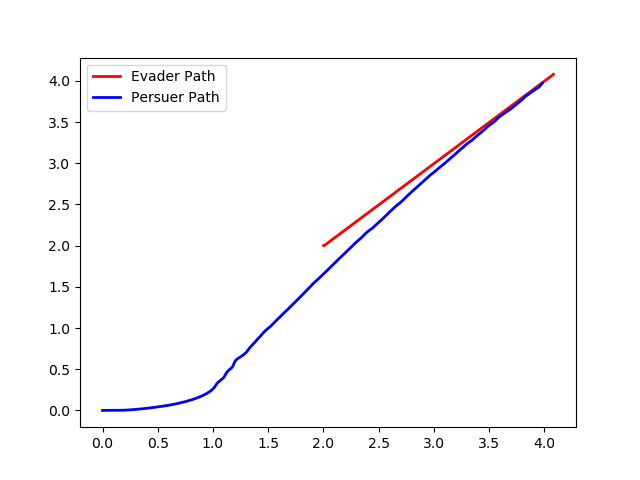
\includegraphics[width=0.7\textwidth]{images/question1.png}
\caption{Evader and Pursuer Position Plot}
\label{fig:question1}
\end{figure}

\bigskip
\noindent My pursuer intercepted the target just a few seconds before the 30 second mark. I used a PN constant of 1.5


\section*{Problem 2}
With the evader moving from [2,2] to [9,9], test out your working pursuit script. Although random 
between tests, perform 3 tests with PN constant = 10\% of problem 1 value, 100\%, and 1000\%. 
How does the performance change in in terms of capturing the random evader? Provide 
plots/figures to support what you see.

\bigskip
\begin{figure}[H]
\centering
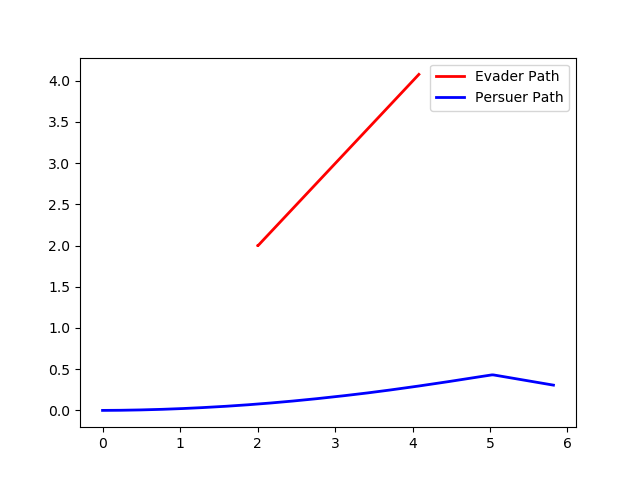
\includegraphics[width=0.7\textwidth]{images/question2a.png}
\caption{Evader and Pursuer Position Plot with 10\% Gain}
\label{fig:question2}
\end{figure}

\bigskip
\noindent The pursuer was not able to intercept the target with a gain of 10\% as seen above. It just didn't turn quickly enough.



\begin{figure}[H]
\centering
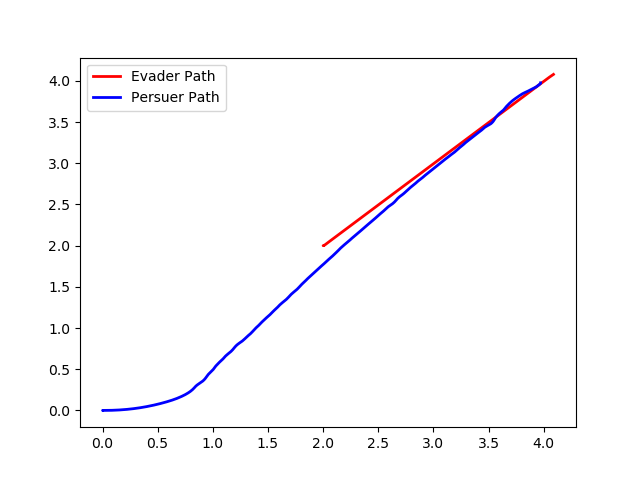
\includegraphics[width=0.7\textwidth]{images/question2b.png}
\caption{Evader and Pursuer Position Plot with 100\% Gain}
\label{fig:question2}
\end{figure}

\bigskip
\noindent As we had previously seen, and expect, the pursuer did just fine at the 100\% gain.


\begin{figure}[H]
\centering
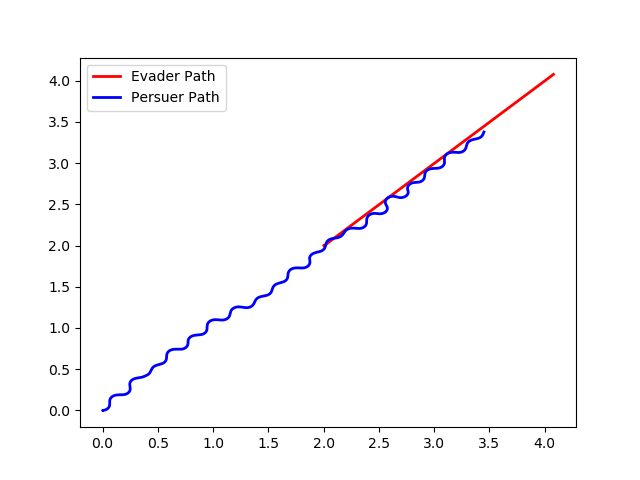
\includegraphics[width=0.7\textwidth]{images/question2c.png}
\caption{Evader and Pursuer Position Plot with 1000\% Gain}
\label{fig:question2}
\end{figure}

\bigskip
\noindent Using a gain of 1000\% was a bit too much. The pursuer was able to intercept the target, but it took longer than 30 seconds and is not shown. It took a very "wiggly" adjusting too aggressively with sharp turns.

\section*{Problem 3}

With the evader moving randomly ,test out your pursuit script. Comment on how it performs (run 
this simulation a few times to compare). Provide plots/figures to support what you see).

subfigures 

\bigskip
\begin{figure}[H]
    \begin{subfigure}[b]{0.5\textwidth}
        \centering
        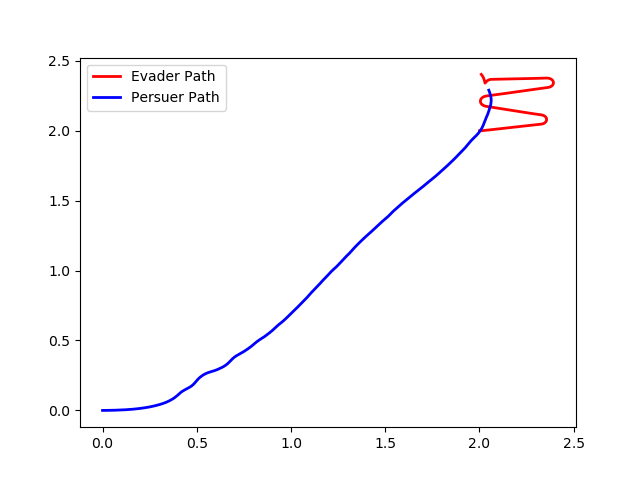
\includegraphics[width=0.7\textwidth]{images/question3a.png}
        \label{fig:question3a}
    \end{subfigure}
    \begin{subfigure}[b]{0.5\textwidth}
        \centering
        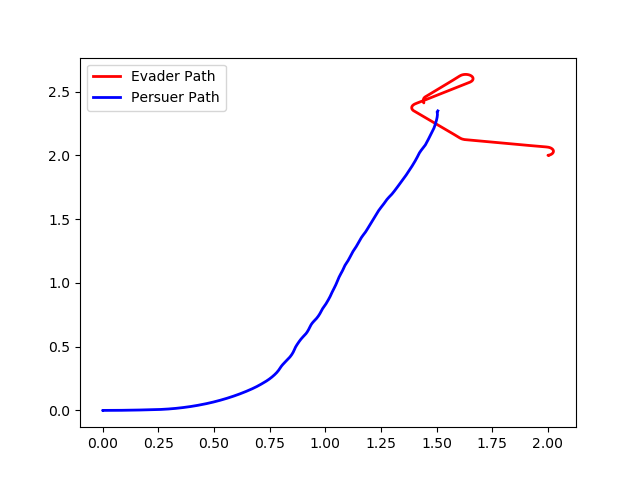
\includegraphics[width=0.7\textwidth]{images/question3b.png}
        \label{fig:question3b}
    \end{subfigure}
    \begin{subfigure}[b]{0.5\textwidth}
        \centering
        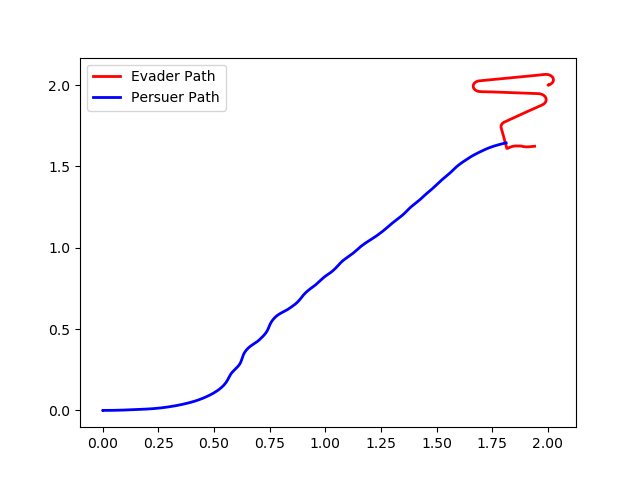
\includegraphics[width=0.7\textwidth]{images/question3c.png}
        \label{fig:question3c}
    \end{subfigure}
    \caption{Evader and Pursuer Position Plots}
    \label{fig:question3}
\end{figure}

\bigskip
\noindent The pursuer was able to intercept the target in every case. It would seem random wondering wasn't sufficient to trick the PN.

\section*{Problem 4}

Using an evader with a maximum speed of 0.1 m/s (and your own pursuer of 0.2 m/s) and a starting 
location of (2,2) and a goal location of (9,9), create an evader that can out-maneuver your pursuer
(pursuer starts at (0,0).

\bigskip
\begin{figure}[H]
\centering
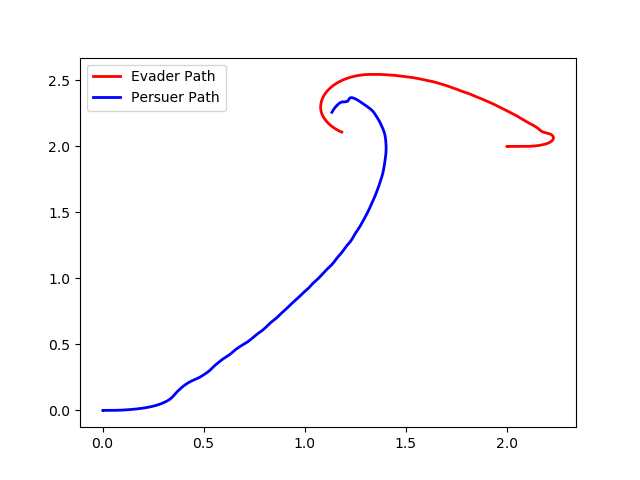
\includegraphics[width=0.7\textwidth]{images/question4.png}
\caption{Evader and Pursuer Position Plot}
\label{fig:question4}
\end{figure}

\bigskip
\noindent I was occasionally able to evade the pursuer by having the evader uses proportional navigation, but offsetting the percieved angle by 90 degrees. When the pursuer got close, my evader would try to turn sharp and circle around the evader. It was succesful on some runs, but was inconsistent and only worked a fraction of the time.

\section*{Problem 5}

Work with a partner to test your evader and pursuer (take turns) identical to Problem 4. You can 
accomplish this through sharing scripts or by connecting two machines in ROS2. See the link below 
for a quick tutorial on how to do this (quite easy).
https://roboticsbackend.com/ros2-multiple-machines-including-raspberry-pi/
Show plots of your pursuer and evader

\bigskip

\begin{figure}[H]
\centering
\begin {subfigure}[b]{0.5\textwidth}
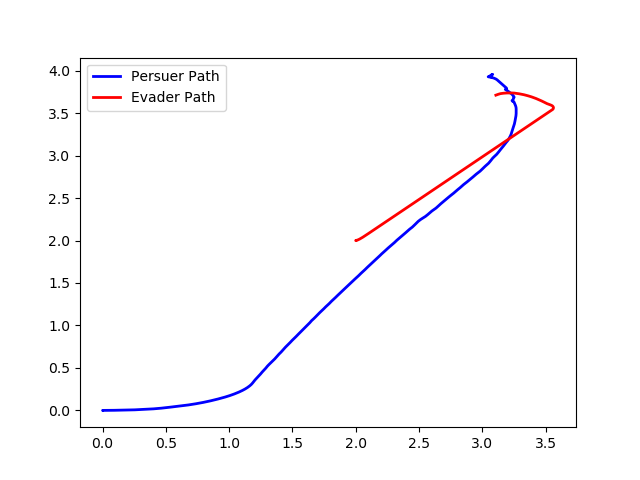
\includegraphics[width=0.7\textwidth]{question5a_my_pursuer.png}
\caption*{My Pursuer against Chris' Evader}
\label{fig:question5a}
\end{subfigure}
\begin {subfigure}[b]{0.5\textwidth}
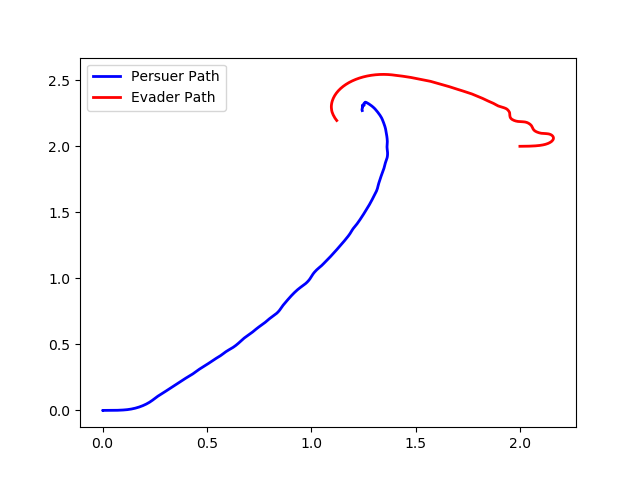
\includegraphics[width=0.7\textwidth]{question5b_my_evader.png}
\caption*{Chris' Pursuer against My Evader}
\label{fig:question5b}
\end{subfigure}
\label{fig:question5}
\end{figure}

\bigskip
\noindent The story was similar to question 4. I was always able to intercept Chris's evader. My evader was sometimes able to evade Chris's purserer for a moment, getting behind him, but it would catch up later, and slam into my evader.

\end{document}